\usepackage{animate}
\usepackage{media9}
\usepackage{tikz}
\usepackage{ifthen}
\usepackage{xcolor}

\usepackage[absolute,overlay]{textpos}

\DeclareSymbolFont{extraup}{U}{zavm}{m}{n}
\DeclareMathSymbol{\varheart}{\mathalpha}{extraup}{86}
\DeclareMathSymbol{\vardiamond}{\mathalpha}{extraup}{87}

% Actually draw the card
% This will be called from within a tikz environment within a appropriatley
% shifted scope. Draw the card in the rectangle between (0,0) and (1,-1.4).
% Arguments:
%     #1 suit (clubs: 0, diamond: 1, heart: 2, spade: 3)
%     #2 value (ace: 1, 2-10, jack: 11, queen: 12, king: 13)
%     #3 selected (0 or 1)
% Keep this short, as it will be called thousands of times
\definecolor{selectedcolor}{RGB}{173,255,189}
\newcommand*{\doDrawCard}[3]{
    \ifthenelse{#3=1}{
        \draw[rounded corners=5pt,fill=selectedcolor] (0,0) rectangle ++(1,-1.4);
    }{
        \draw[rounded corners=5pt,fill=white] (0,0) rectangle ++(1,-1.4);
    }
    %\draw (0,-0.7) -- ++(1,0);
    %\draw (0,0) rectangle ++(1,-1.4);
    \ifthenelse{#1=0 \or #1=3}{
        \node[text centered,text width=1cm,below] at (0.5,0) {\getValue{#2}~\getSuit{#1}};
        \node[text centered,text width=1cm,below,rotate=180] at (0.5,-1.4) {\getValue{#2}~\getSuit{#1}};
    }{
        \node[text centered,text width=1cm,below,red] at (0.5,0) {\getValue{#2}~\getSuit{#1}};
        \node[text centered,text width=1cm,below,red,rotate=180] at (0.5,-1.4) {\getValue{#2}~\getSuit{#1}};
    }
}

\newcommand*{\drawMode}[1]{
    \begin{tikzpicture}
        \path[draw, use as bounding box] (0,0) rectangle ++(1,-1);
        \ifthenelse{#1=0}{
            \node at (0.5,-0.5) {\getSuit{0}};
        }{
            \ifthenelse{#1=1}{
                \node at (0.5,-0.5) {\getSuit{0}\getSuit{1}};
            }{
                \node[text centered, text width=1cm] at (0.5,-0.5) {\getSuit{0}~\getSuit{1}\\\getSuit{2}~\getSuit{3}};
            }
        }
    \end{tikzpicture}
}

\newcommand*{\getSuit}[1]{%
    \ifthenelse{#1=0}{$\clubsuit$}{\ifthenelse{#1=1}{$\vardiamond$}{\ifthenelse{#1=2}{$\varheart$}{$\spadesuit$}}}%
}
\newcommand*{\getValue}[1]{%
    \ifthenelse{#1=1}{A}{\ifthenelse{#1=11}{J}{\ifthenelse{#1=12}{Q}{\ifthenelse{#1=13}{K}{#1}}}}%
}


\textblockorigin{1cm}{1.5cm}
\setlength{\TPHorizModule}{1.1cm}
\setlength{\TPVertModule}{1cm}

% helper function for drawing card
\newcommand*{\drawCard}[5]{ % column, index, suit, value
    \begin{tikzpicture}
        \path[use as bounding box] (0,2) rectangle (8.7,-10);
        \ifthenelse{#4=0}{}{
            \begin{scope}[shift={(#1*1.1,-#2*0.5)}]
                \doDrawCard{#3}{#4}{#5}
            \end{scope}
        }
    \end{tikzpicture}
}

% draw button area
\newcommand*{\drawColumnButton}{
    \begin{tikzpicture}
        \path[use as bounding box] (0,0) rectangle (0.88,-10);
    \end{tikzpicture}
}
\newcommand*{\drawCardButton}{
    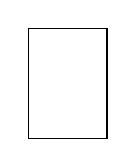
\begin{tikzpicture}
        \path[draw] (0,0) rectangle ++(1,-1.4);
    \end{tikzpicture}
}
\newcommand*{\drawGameButton}[1]{
    \begin{tikzpicture}
        \path[draw,use as bounding box] (0,0) rectangle ++(2,-1);
        \node at (1,-0.5) {#1};
    \end{tikzpicture}
}

% helper function to create animate object for a card
\newcommand*{\doMakeCard}[3]{ % column, index, label
    \begin{textblock}{2}[0,0](0,0)
        \begin{animateinline}[label=#3,nomouse]{1}
            \drawCard{#1}{#2}{0}{0}{0} \newframe
            %
            \drawCard{#1}{#2}{0}{1}{0} \newframe
            \drawCard{#1}{#2}{0}{2}{0} \newframe
            \drawCard{#1}{#2}{0}{3}{0} \newframe
            \drawCard{#1}{#2}{0}{4}{0} \newframe
            \drawCard{#1}{#2}{0}{5}{0} \newframe
            \drawCard{#1}{#2}{0}{6}{0} \newframe
            \drawCard{#1}{#2}{0}{7}{0} \newframe
            \drawCard{#1}{#2}{0}{8}{0} \newframe
            \drawCard{#1}{#2}{0}{9}{0} \newframe
            \drawCard{#1}{#2}{0}{10}{0} \newframe
            \drawCard{#1}{#2}{0}{11}{0} \newframe
            \drawCard{#1}{#2}{0}{12}{0} \newframe
            \drawCard{#1}{#2}{0}{13}{0} \newframe
            %
            \drawCard{#1}{#2}{1}{1}{0} \newframe
            \drawCard{#1}{#2}{1}{2}{0} \newframe
            \drawCard{#1}{#2}{1}{3}{0} \newframe
            \drawCard{#1}{#2}{1}{4}{0} \newframe
            \drawCard{#1}{#2}{1}{5}{0} \newframe
            \drawCard{#1}{#2}{1}{6}{0} \newframe
            \drawCard{#1}{#2}{1}{7}{0} \newframe
            \drawCard{#1}{#2}{1}{8}{0} \newframe
            \drawCard{#1}{#2}{1}{9}{0} \newframe
            \drawCard{#1}{#2}{1}{10}{0} \newframe
            \drawCard{#1}{#2}{1}{11}{0} \newframe
            \drawCard{#1}{#2}{1}{12}{0} \newframe
            \drawCard{#1}{#2}{1}{13}{0} \newframe
            %
            \drawCard{#1}{#2}{2}{1}{0} \newframe
            \drawCard{#1}{#2}{2}{2}{0} \newframe
            \drawCard{#1}{#2}{2}{3}{0} \newframe
            \drawCard{#1}{#2}{2}{4}{0} \newframe
            \drawCard{#1}{#2}{2}{5}{0} \newframe
            \drawCard{#1}{#2}{2}{6}{0} \newframe
            \drawCard{#1}{#2}{2}{7}{0} \newframe
            \drawCard{#1}{#2}{2}{8}{0} \newframe
            \drawCard{#1}{#2}{2}{9}{0} \newframe
            \drawCard{#1}{#2}{2}{10}{0} \newframe
            \drawCard{#1}{#2}{2}{11}{0} \newframe
            \drawCard{#1}{#2}{2}{12}{0} \newframe
            \drawCard{#1}{#2}{2}{13}{0} \newframe
            %
            \drawCard{#1}{#2}{3}{1}{0} \newframe
            \drawCard{#1}{#2}{3}{2}{0} \newframe
            \drawCard{#1}{#2}{3}{3}{0} \newframe
            \drawCard{#1}{#2}{3}{4}{0} \newframe
            \drawCard{#1}{#2}{3}{5}{0} \newframe
            \drawCard{#1}{#2}{3}{6}{0} \newframe
            \drawCard{#1}{#2}{3}{7}{0} \newframe
            \drawCard{#1}{#2}{3}{8}{0} \newframe
            \drawCard{#1}{#2}{3}{9}{0} \newframe
            \drawCard{#1}{#2}{3}{10}{0} \newframe
            \drawCard{#1}{#2}{3}{11}{0} \newframe
            \drawCard{#1}{#2}{3}{12}{0} \newframe
            \drawCard{#1}{#2}{3}{13}{0} \newframe
            %
            \drawCard{#1}{#2}{0}{1}{1} \newframe
            \drawCard{#1}{#2}{0}{2}{1} \newframe
            \drawCard{#1}{#2}{0}{3}{1} \newframe
            \drawCard{#1}{#2}{0}{4}{1} \newframe
            \drawCard{#1}{#2}{0}{5}{1} \newframe
            \drawCard{#1}{#2}{0}{6}{1} \newframe
            \drawCard{#1}{#2}{0}{7}{1} \newframe
            \drawCard{#1}{#2}{0}{8}{1} \newframe
            \drawCard{#1}{#2}{0}{9}{1} \newframe
            \drawCard{#1}{#2}{0}{10}{1} \newframe
            \drawCard{#1}{#2}{0}{11}{1} \newframe
            \drawCard{#1}{#2}{0}{12}{1} \newframe
            \drawCard{#1}{#2}{0}{13}{1} \newframe
            %
            \drawCard{#1}{#2}{1}{1}{1} \newframe
            \drawCard{#1}{#2}{1}{2}{1} \newframe
            \drawCard{#1}{#2}{1}{3}{1} \newframe
            \drawCard{#1}{#2}{1}{4}{1} \newframe
            \drawCard{#1}{#2}{1}{5}{1} \newframe
            \drawCard{#1}{#2}{1}{6}{1} \newframe
            \drawCard{#1}{#2}{1}{7}{1} \newframe
            \drawCard{#1}{#2}{1}{8}{1} \newframe
            \drawCard{#1}{#2}{1}{9}{1} \newframe
            \drawCard{#1}{#2}{1}{10}{1} \newframe
            \drawCard{#1}{#2}{1}{11}{1} \newframe
            \drawCard{#1}{#2}{1}{12}{1} \newframe
            \drawCard{#1}{#2}{1}{13}{1} \newframe
            %
            \drawCard{#1}{#2}{2}{1}{1} \newframe
            \drawCard{#1}{#2}{2}{2}{1} \newframe
            \drawCard{#1}{#2}{2}{3}{1} \newframe
            \drawCard{#1}{#2}{2}{4}{1} \newframe
            \drawCard{#1}{#2}{2}{5}{1} \newframe
            \drawCard{#1}{#2}{2}{6}{1} \newframe
            \drawCard{#1}{#2}{2}{7}{1} \newframe
            \drawCard{#1}{#2}{2}{8}{1} \newframe
            \drawCard{#1}{#2}{2}{9}{1} \newframe
            \drawCard{#1}{#2}{2}{10}{1} \newframe
            \drawCard{#1}{#2}{2}{11}{1} \newframe
            \drawCard{#1}{#2}{2}{12}{1} \newframe
            \drawCard{#1}{#2}{2}{13}{1} \newframe
            %
            \drawCard{#1}{#2}{3}{1}{1} \newframe
            \drawCard{#1}{#2}{3}{2}{1} \newframe
            \drawCard{#1}{#2}{3}{3}{1} \newframe
            \drawCard{#1}{#2}{3}{4}{1} \newframe
            \drawCard{#1}{#2}{3}{5}{1} \newframe
            \drawCard{#1}{#2}{3}{6}{1} \newframe
            \drawCard{#1}{#2}{3}{7}{1} \newframe
            \drawCard{#1}{#2}{3}{8}{1} \newframe
            \drawCard{#1}{#2}{3}{9}{1} \newframe
            \drawCard{#1}{#2}{3}{10}{1} \newframe
            \drawCard{#1}{#2}{3}{11}{1} \newframe
            \drawCard{#1}{#2}{3}{12}{1} \newframe
            \drawCard{#1}{#2}{3}{13}{1}
        \end{animateinline}
    \end{textblock}
}

% create regular card a position
\newcommand*{\makeCard}[2]{         % column, index
    \doMakeCard{#1}{#2}{c#1x#2}
}

% create card with custom label and action
\newcommand*{\makeSpecialCard}[3]{  % column, index, label
    \doMakeCard{#1}{#2/0.5}{#3}
}

\newcommand*{\makeButton}[1]{   % column
    \begin{textblock}{2}(#1,2)
        \mediabutton[jsaction={
            if(typeof(column_clicked) != "undefined")
                column_clicked(#1);
        }]{%
            \hspace*{-0.12cm}%
            \drawColumnButton
        }
    \end{textblock}
}

\newcommand*{\makeCardButton}[3]{   % column, index, action
    \begin{textblock}{2}(#1,0)
        \mediabutton[jsaction={
            if(typeof(special_clicked) != "undefined")
                special_clicked("#3");
        }]{%
            \hspace*{-0.12cm}%
            \drawCardButton
        }
    \end{textblock}
}

\newcommand*{\makeGameButton}[4]{   % column, index, text, action
    \begin{textblock}{2}(#1,#2)
        \mediabutton[jsaction={
            #4
        }]{%
            \hspace*{-0.12cm}%
            \drawGameButton{#3}
        }
    \end{textblock}
}

\newcommand*{\drawBackground}{
    \definecolor{tablecolor}{RGB}{62, 114, 17}
    \begin{textblock}{2}[0,0](-1,-1)
        \begin{tikzpicture}
            \path[use as bounding box,draw,fill=tablecolor] (0,2) rectangle (10.9,-12);
        \end{tikzpicture}
    \end{textblock}
}
